\documentclass[tikz,border=8pt]{standalone}
\usepackage{amsmath}
\usetikzlibrary{arrows.meta,calc,decorations.pathreplacing}
\definecolor{ink}{HTML}{21352F}
\definecolor{teal}{HTML}{087F7B}
\definecolor{gold}{HTML}{C58B2A}
\definecolor{blue}{HTML}{4B77A8}
\definecolor{rose}{HTML}{B65A62}
\definecolor{paper}{HTML}{FFFCF6}
\begin{document}
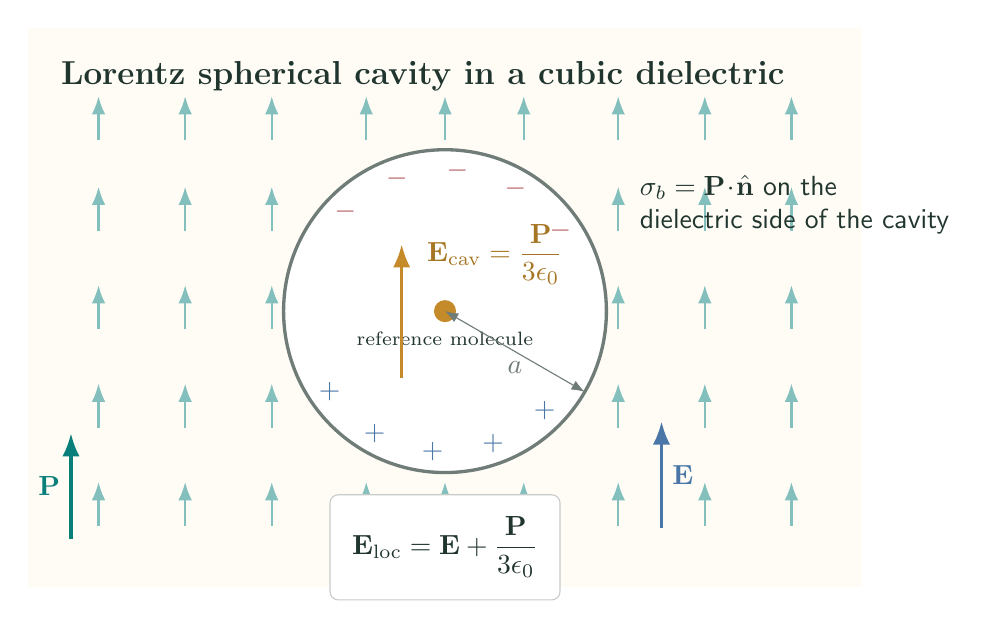
\begin{tikzpicture}[font=\sffamily,text=ink,>=Latex]
  \fill[paper] (-5.3,-3.5) rectangle (5.3,3.6);
  \node[anchor=north west,font=\bfseries\large] at (-5.0,3.3) {Lorentz spherical cavity in a cubic dielectric};
  \foreach \x in {-4.4,-3.3,-2.2,2.2,3.3,4.4}
    \foreach \y in {-2.45,-1.2,0.05,1.3,2.45}
      \draw[->,teal!50,thick] (\x,\y-0.28)--(\x,\y+0.28);
  \foreach \x in {-1.0,0,1.0}
    \foreach \y in {-2.45,2.45}
      \draw[->,teal!50,thick] (\x,\y-0.28)--(\x,\y+0.28);
  \draw[ink!65,very thick,fill=white] (0,0) circle (2.05);
  \fill[gold] (0,0) circle (0.14);
  \node[below=4pt,font=\scriptsize] at (0,0) {reference molecule};
  \draw[<->,ink!65] (0,0)--(330:2.05) node[midway,below] {$a$};
  \foreach \ang in {35,60,85,110,135}{\node[rose,font=\bfseries] at (\ang:1.79) {$-$};}
  \foreach \ang in {215,240,265,290,315}{\node[blue,font=\bfseries] at (\ang:1.79) {$+$};}
  \draw[->,very thick,teal] (-4.75,-2.9)--(-4.75,-1.55) node[midway,left] {$\mathbf P$};
  \draw[->,very thick,blue] (2.75,-2.75)--(2.75,-1.40) node[midway,right] {$\mathbf E$};
  \draw[->,very thick,gold] (-0.55,-0.85)--(-0.55,0.85);
  \node[anchor=west,gold!85!black] at (-0.35,0.72) {$\mathbf E_{\rm cav}=\dfrac{\mathbf P}{3\epsilon_0}$};
  \node[align=left,anchor=west] at (2.35,1.35) {$\sigma_b=\mathbf P\!\cdot\!\hat{\mathbf n}$ on the\\dielectric side of the cavity};
  \node[draw=ink!25,rounded corners=3pt,fill=white,inner sep=8pt] at (0,-3.0) {$\displaystyle \mathbf E_{\rm loc}=\mathbf E+\frac{\mathbf P}{3\epsilon_0}$};
\end{tikzpicture}
\end{document}
